\documentclass{standalone}
\usepackage{tikz}
\usetikzlibrary{patterns, positioning}

\begin{document}
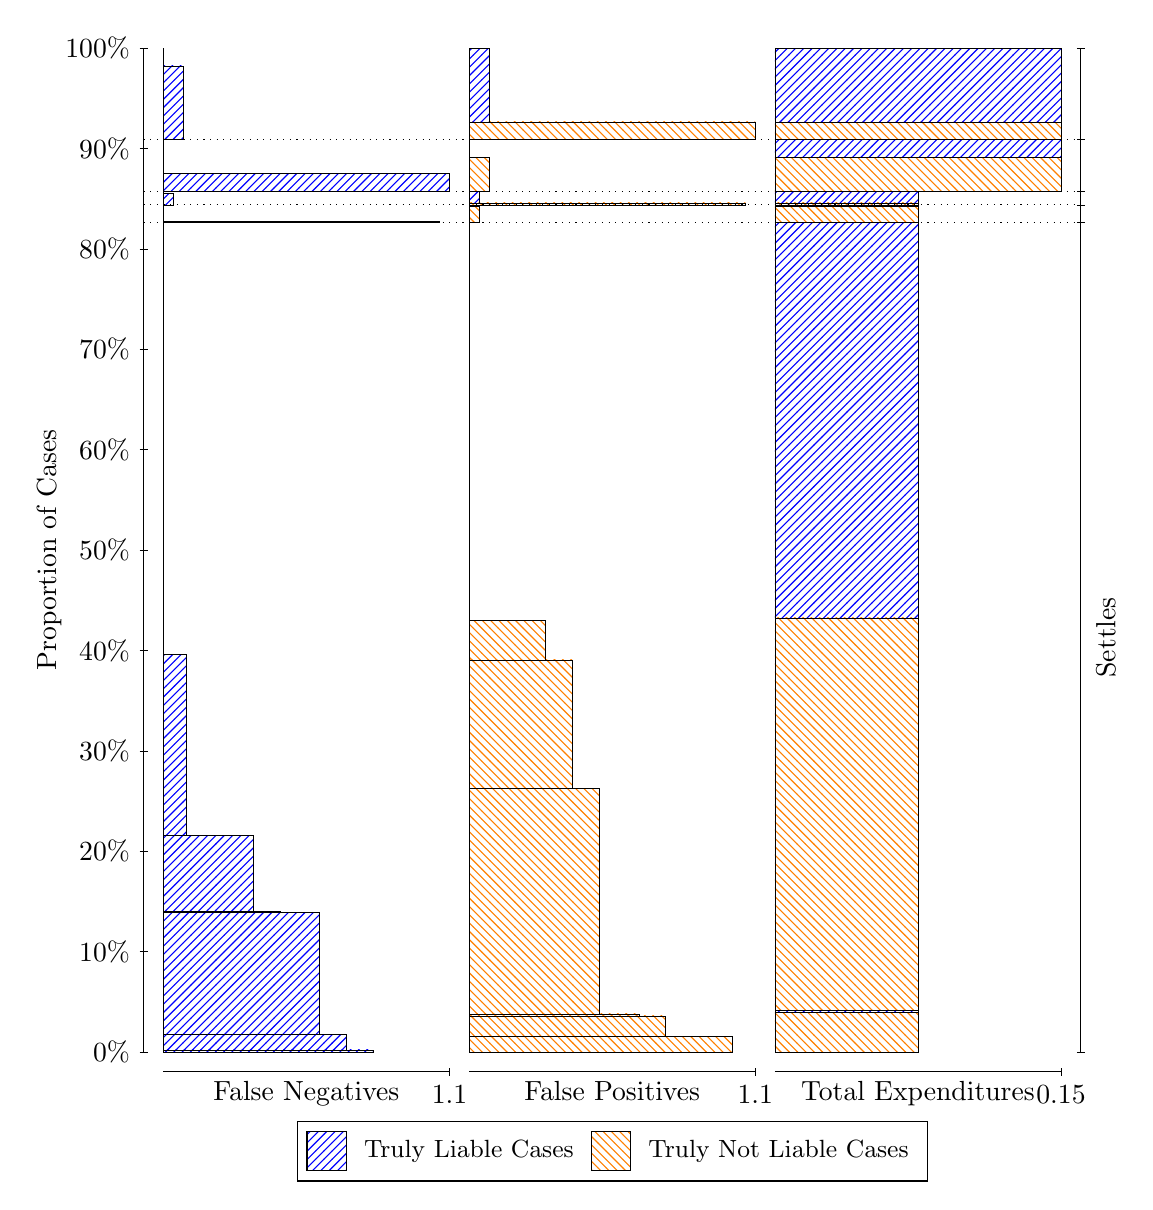
\begin{tikzpicture}
\draw[black, very thin] (1.5,1.75) -- (1.5,14.5);
\node[rotate=90, anchor=center] at (0.3, 8.125) {Proportion of Cases};
\draw[black, very thin] (1.45,1.75) -- (1.55,1.75);
\node[anchor=east] at (1.45, 1.75) {0\%};
\draw[black, very thin] (1.45,3.025) -- (1.55,3.025);
\node[anchor=east] at (1.45, 3.025) {10\%};
\draw[black, very thin] (1.45,4.3) -- (1.55,4.3);
\node[anchor=east] at (1.45, 4.3) {20\%};
\draw[black, very thin] (1.45,5.575) -- (1.55,5.575);
\node[anchor=east] at (1.45, 5.575) {30\%};
\draw[black, very thin] (1.45,6.85) -- (1.55,6.85);
\node[anchor=east] at (1.45, 6.85) {40\%};
\draw[black, very thin] (1.45,8.125) -- (1.55,8.125);
\node[anchor=east] at (1.45, 8.125) {50\%};
\draw[black, very thin] (1.45,9.4) -- (1.55,9.4);
\node[anchor=east] at (1.45, 9.4) {60\%};
\draw[black, very thin] (1.45,10.675) -- (1.55,10.675);
\node[anchor=east] at (1.45, 10.675) {70\%};
\draw[black, very thin] (1.45,11.95) -- (1.55,11.95);
\node[anchor=east] at (1.45, 11.95) {80\%};
\draw[black, very thin] (1.45,13.225) -- (1.55,13.225);
\node[anchor=east] at (1.45, 13.225) {90\%};
\draw[black, very thin] (1.45,14.5) -- (1.55,14.5);
\node[anchor=east] at (1.45, 14.5) {100\%};

\draw[black, very thin] (13.4,1.75) -- (13.4,14.5);
\draw[black, very thin] (13.35,1.75) -- (13.45,1.75);
\node[anchor=west] at (13.35, 1.75) {};
\draw[black, very thin] (13.35,12.282) -- (13.45,12.282);
\node[anchor=west] at (13.35, 12.282) {};
\draw[black, very thin] (13.35,12.509) -- (13.45,12.509);
\node[anchor=west] at (13.35, 12.509) {};
\draw[black, very thin] (13.35,12.679) -- (13.45,12.679);
\node[anchor=west] at (13.35, 12.679) {};
\draw[black, very thin] (13.35,13.336) -- (13.45,13.336);
\node[anchor=west] at (13.35, 13.336) {};
\draw[black, very thin] (13.35,14.5) -- (13.45,14.5);
\node[anchor=west] at (13.35, 14.5) {};

\draw[black, very thin, pattern color=blue, pattern=north east lines] (1.75,1.75) rectangle (4.4116,1.7777);
\draw[black, very thin, pattern color=blue, pattern=north east lines] (1.75,1.7777) rectangle (4.0736,1.9717);
\draw[black, very thin, pattern color=blue, pattern=north east lines] (1.75,1.9717) rectangle (3.7357,3.5206);
\draw[black, very thin, pattern color=blue, pattern=north east lines] (1.75,3.5206) rectangle (3.2287,3.54);
\draw[black, very thin, pattern color=blue, pattern=north east lines] (1.75,3.54) rectangle (2.8907,4.5028);
\draw[black, very thin, pattern color=blue, pattern=north east lines] (1.75,4.5028) rectangle (2.0457,6.7978);
\draw[black, very thin, pattern color=orange, pattern=north west lines] (1.75,6.7978) rectangle (1.75,12.282);
\draw[black, very thin, pattern color=blue, pattern=north east lines] (1.75,12.282) rectangle (5.2566,12.298);
\draw[black, very thin, pattern color=orange, pattern=north west lines] (1.75,12.298) rectangle (1.75,12.509);
\draw[black, very thin, pattern color=blue, pattern=north east lines] (1.75,12.509) rectangle (1.8767,12.655);
\draw[black, very thin, pattern color=orange, pattern=north west lines] (1.75,12.655) rectangle (1.75,12.679);
\draw[black, very thin, pattern color=blue, pattern=north east lines] (1.75,12.679) rectangle (5.3833,12.907);
\draw[black, very thin, pattern color=orange, pattern=north west lines] (1.75,12.907) rectangle (1.75,13.336);
\draw[black, very thin, pattern color=blue, pattern=north east lines] (1.75,13.336) rectangle (2.0035,14.273);
\draw[black, very thin, pattern color=orange, pattern=north west lines] (1.75,14.273) rectangle (1.75,14.5);
\draw[black, very thin, pattern color=orange, pattern=north west lines] (5.6333,1.75) rectangle (8.9709,1.9486);
\draw[black, very thin, pattern color=orange, pattern=north west lines] (5.6333,1.9486) rectangle (8.126,2.2077);
\draw[black, very thin, pattern color=orange, pattern=north west lines] (5.6333,2.2077) rectangle (7.788,2.2345);
\draw[black, very thin, pattern color=orange, pattern=north west lines] (5.6333,2.2345) rectangle (7.281,5.1012);
\draw[black, very thin, pattern color=orange, pattern=north west lines] (5.6333,5.1012) rectangle (6.943,6.7306);
\draw[black, very thin, pattern color=orange, pattern=north west lines] (5.6333,6.7306) rectangle (6.605,7.2341);
\draw[black, very thin, pattern color=blue, pattern=north east lines] (5.6333,7.2341) rectangle (5.6333,12.282);
\draw[black, very thin, pattern color=orange, pattern=north west lines] (5.6333,12.282) rectangle (5.7601,12.493);
\draw[black, very thin, pattern color=blue, pattern=north east lines] (5.6333,12.493) rectangle (5.6333,12.509);
\draw[black, very thin, pattern color=orange, pattern=north west lines] (5.6333,12.509) rectangle (9.1399,12.533);
\draw[black, very thin, pattern color=blue, pattern=north east lines] (5.6333,12.533) rectangle (5.7601,12.679);
\draw[black, very thin, pattern color=orange, pattern=north west lines] (5.6333,12.679) rectangle (5.8868,13.109);
\draw[black, very thin, pattern color=blue, pattern=north east lines] (5.6333,13.109) rectangle (5.6333,13.336);
\draw[black, very thin, pattern color=orange, pattern=north west lines] (5.6333,13.336) rectangle (9.2667,13.563);
\draw[black, very thin, pattern color=blue, pattern=north east lines] (5.6333,13.563) rectangle (5.8868,14.5);
\draw[black, very thin, pattern color=orange, pattern=north west lines] (9.5167,1.75) rectangle (11.333,2.2535);
\draw[black, very thin, pattern color=blue, pattern=north east lines] (9.5167,2.2535) rectangle (11.333,2.2812);
\draw[black, very thin, pattern color=orange, pattern=north west lines] (9.5167,2.2812) rectangle (11.333,7.2618);
\draw[black, very thin, pattern color=blue, pattern=north east lines] (9.5167,7.2618) rectangle (11.333,12.282);
\draw[black, very thin, pattern color=orange, pattern=north west lines] (9.5167,12.282) rectangle (11.333,12.493);
\draw[black, very thin, pattern color=blue, pattern=north east lines] (9.5167,12.493) rectangle (11.333,12.509);
\draw[black, very thin, pattern color=orange, pattern=north west lines] (9.5167,12.509) rectangle (11.333,12.533);
\draw[black, very thin, pattern color=blue, pattern=north east lines] (9.5167,12.533) rectangle (11.333,12.679);
\draw[black, very thin, pattern color=orange, pattern=north west lines] (9.5167,12.679) rectangle (13.15,13.109);
\draw[black, very thin, pattern color=blue, pattern=north east lines] (9.5167,13.109) rectangle (13.15,13.336);
\draw[black, very thin, pattern color=orange, pattern=north west lines] (9.5167,13.336) rectangle (13.15,13.563);
\draw[black, very thin, pattern color=blue, pattern=north east lines] (9.5167,13.563) rectangle (13.15,14.5);
\draw[black, dotted] (1.5,12.282) -- (13.4,12.282);
\draw[black, dotted] (1.5,12.509) -- (13.4,12.509);
\draw[black, dotted] (1.5,12.679) -- (13.4,12.679);
\draw[black, dotted] (1.5,13.336) -- (13.4,13.336);
\draw[black, very thin] (1.75,1.5) -- (5.3833,1.5);
\node[anchor=north] at (3.5667, 1.5) {False Negatives};
\draw[black, very thin] (5.3833,1.45) -- (5.3833,1.55);
\node[anchor=north] at (5.3833, 1.45) {1.1};

\draw[black, very thin] (5.6333,1.5) -- (9.2667,1.5);
\node[anchor=north] at (7.45, 1.5) {False Positives};
\draw[black, very thin] (9.2667,1.45) -- (9.2667,1.55);
\node[anchor=north] at (9.2667, 1.45) {1.1};

\draw[black, very thin] (9.5167,1.5) -- (13.15,1.5);
\node[anchor=north] at (11.333, 1.5) {Total Expenditures};
\draw[black, very thin] (13.15,1.45) -- (13.15,1.55);
\node[anchor=north] at (13.15, 1.45) {0.15};

\node[black, centered, rotate=90] at (13.72, 7.016) {Settles};





\draw (7.449999999999999,1.5) node[draw=none] (baseCoordinate) {};
\begin{scope}[align=center]
        \matrix[scale=0.5, draw=black, below=0.5cm of baseCoordinate, nodes={draw}, column sep=0.1cm]{
            \node[rectangle, draw, minimum width=0.5cm, minimum height=0.5cm, pattern=north east lines, pattern color=blue] {}; &
            \node[draw=none, font=\small] (B) {Truly Liable Cases}; &
            \node[rectangle, draw, minimum width=0.5cm, minimum height=0.5cm, pattern=north west lines, pattern color=orange] {}; &
            \node[draw=none, font=\small] (B) {Truly Not Liable Cases}; \\
            };
\end{scope}

\end{tikzpicture}
\end{document}